\documentclass[epsfig,10pt,fullpage]{article}

\newcommand{\LabNum}{9}
\newcommand{\CommonDocsPath}{../../common/docs}
\addtolength{\textwidth}{1.5in}
\addtolength{\oddsidemargin}{-0.75in}
\addtolength{\topmargin}{-0.75in}
\addtolength{\textheight}{1.5in}
\addtolength{\evensidemargin}{0.75in}
\setlength\parindent{0pt}
\raggedbottom

\usepackage{ae,aecompl}
\usepackage{epsfig,float,times}
\usepackage[hypcap]{caption}
\usepackage[pdftex, colorlinks]{hyperref}
\usepackage{graphicx}
\usepackage[usenames, dvipsnames]{color}
\usepackage{rotating}
\usepackage{tikz}
\usetikzlibrary{automata,positioning}
\usepackage{placeins}

\widowpenalty 10000
\clubpenalty 10000

\newcommand{\red}[1]{{\color{red}\sf{#1}}}
\newcommand{\green}[1]{{\color{green}\sf{#1}}}
\newcommand{\blue}[1]{{\color{blue}\sf{#1}}}
\definecolor{PineGreen}{rgb}{0.0, 0.47, 0.44}
\definecolor{ForestGreen}{rgb}{0.13, 0.55, 0.13}
\definecolor{Brown}{rgb}{0.59, 0.29, 0.0}

\newcommand{\UPDatePublished}{Oct 2021}
\newcommand{\versnum}{21.1} %version number quartus/AMP
\newcommand{\quartusname}{Quartus\textsuperscript{\textregistered} Prime}	
\newcommand{\UPTextBar}{For \quartusname{} \versnum{}}
\newcommand{\thisyear}{2021 } %for copyright
\newcommand{\company}{FPGAcademy.org}
\newcommand{\longteamname}{FPGAcademy.org}
\newcommand{\teamname}{FPGAcademy}
\newcommand{\website}{FPGAcademy.org}

\newcommand{\productAcronym}{AMP}
\newcommand{\productNameShort}{Monitor Program}

\newcommand{\productNameMedTM}{A Monitor Program}
\newcommand{\productNameMed}{A Monitor Program}

%\newcommand{\headerLogoFilePath}[1]{#1/FPGAcademy.png}

% listings is a package that supports encapsulating source code in LaTeX conveniently
\usepackage{listings}

\def\expandparam\lstinputlisting[#1]#2{\edef\tmp{\noexpand\lstinputlisting[#1]{#2}}\tmp}

%%%%%%%%%%%%%%%%%%%% Source Code Formatting %%%%%%%%%%%%%%%%%%%%
\definecolor{globalCommentColour}{rgb}{0.588,0.588,0.588}

%%%%%%%%%%%%%%%%%%%%%%%%%%%%%%%%%%%%%%%%%%%%%%%%%%%%
% Defining language style
% NiosII ASM
\lstdefinelanguage[NiosII]{Assembler} {
  morekeywords={add, addi, and, andhi, andi, beq, bge, bgeu, bgt, bgtu, ble,  bleu, blt, bltu, bne, br, break,
  bret, call, callr, cmpeq, cmpeqi, cmpge, cmpgei, cmpgeu, cmpgeui, cmpgt, cmpgti, cmpgtu, cmpgtui, cmple,
  cmplei, cmpleu, cmpleui, cmplt, cmplti, cmpltu, cmpltui, cmpne, cmpnei, custom, div, divu, eret, flushd,
  flushda, flushi, flushp, initd, initda, initi, jmp, jmpi, ldb, ldbio, ldbu, ldbuio, ldh, ldhio, ldhu, ldhuio,
  ldw, ldwio, mov, movhi, movi, movia, movui, mul, muli, mulxss, mulxsu, mulxuu, nextpc, nop, nor, or, orhi, ori,
  rdctl, rdprs, ret, rol, roli, ror, sll, slli, sra, srai, srl, srli, stb, stbio, sth, sthio, stw, stwio,
  sub, subi, sync, trap, wrctl, wrtcl, wrprs, xor, xori, xorhi, xori},
  morekeywords=[2]{.abort, .ABORT, .align, .app-file, .ascii, .asciz, .balign, .byte, .comm, .data, .def,
  .desc, .dim, .double, .eject, .else, .end, .endef, .endif, .equ, .equiv, .err, .extern, .file, .fill, .float,
  .global, .globl, .hword, .ident, .if, .include, .int, .irp, .irpc, .lcomm, .lflags, .line, .linkonce, .ln,
  .list, .long, .macro, .mri, .nolist, .octa, .org, .p2align, .psize, .quad, .rept, .sbttl, .scl, .section,
  .set, .short, .single, .size, .sleb128, .skip, .space, .stadb, .stabn, .stabs, .string, .symver, .tag,
  .text, .title, .type, .val, .uleb128, .word},
  morekeywords=[3]{et, bt, gp, sp, fp, ea, sstatus, ra, pc, status, estatus, bstatus, ienable, ipending, cpuid,
  exception, pteaddr, tlbacc, tlbmisc, eccinj, badaddr, config, mpubase, mpuacc},
  sensitive=t,
  alsoletter=.,
  morestring=[b]",
  morecomment=[s]{/*}{*/},
  morecomment=[l]\#,
}[keywords,comments,strings]
   
%% NOTE: morekeywords=[2] are GNU directives.
   
\definecolor{niosInstructionColour}{rgb}{0.000,0.608,0.000}
\definecolor{niosDirectiveColour}{rgb}{0.000,0.000,0.902}
\definecolor{niosSpecialRegColour}{rgb}{0.000,0.000,0.000}
\definecolor{niosStringColour}{rgb}{0.808,0.482,0.000}
   
%% NOTE: To make bold use: =\bfseries\color{<colour>}
\lstdefinestyle{defaultNiosStyle} {
  language=[NiosII]{Assembler},
  stringstyle=\color{niosStringColour},
  keywordstyle=\color{niosInstructionColour},
  keywordstyle=[2]\color{niosDirectiveColour},
  keywordstyle=[3]\itshape\color{niosSpecialRegColour}
}
%%%%%%%%%%%%%%%%%%%%%%%%%%%%%%%%%%%%%%%%%%%%%%%%%%%%

%%%%%%%%%%%%%%%%%%%%%%%%%%%%%%%%%%%%%%%%%%%%%%%%%%%%
% Defining language style
% ArmA9 ASM
\lstdefinelanguage[ArmA9]{Assembler} {
  morekeywords={ADC, ADD, ADDS, AND, ANDS, B, BAL, BEQ, BGE, BGT, BL, BLT, BIC, BKPT, BLX, BNE, BX, CDP, CLZ, CMN, CMP, EOR,
  EORS, LDC, LDM, LDR, LDRB, LDRBT, LDRH, LDRSB, LDRSH, LDRT, LSL, MCR, MLA, MOV, MOVW, MOVT, MRC, MRS, MSR, MUL, MVN, ORR, PLD,
  ROR, RSB, RSC, SBC, SMLAL, SMULL, STC, STM, STR, STRB, STRBT, STRH, STRT, SUB, SUBS, SWI, SWP, SWPB, TEQ, UMLAL,
  PUSH, POP, MOVS, RORS, LSR},
  morekeywords=[2]{.abort, .ABORT, .align, .app-file, .ascii, .asciz, .balign, .byte, .comm, .data, .def,
  .desc, .dim, .double, .eject, .else, .end, .endef, .endif, .equ, .equiv, .err, .extern, .file, .fill, .float,
  .global, .globl, .hword, .ident, .if, .include, .int, .irp, .irpc, .lcomm, .lflags, .line, .linkonce, .ln,
  .list, .long, .macro, .mri, .nolist, .octa, .org, .p2align, .psize, .quad, .rept, .sbttl, .scl, .section,
  .set, .short, .single, .size, .sleb128, .skip, .space, .stadb, .stabn, .stabs, .string, .symver, .tag,
  .text, .title, .type, .val, .vectors, .uleb128, .word},
  morekeywords=[3]{SP, PC, MIDR, CTR, TCMTR, TLBTR, MPIDR, ID_PFR0, ID_PFR1, ID_DFR0, ID_MMFR0, ID_MMFR1, ID_MMFR2,
  ID_MMFR3, ID_ISAR0, ID_ISAR1, ID_ISAR2, ID_ISAR3, ID_ISAR4, CCSIDR, CLIDR, AIDR, CSSELR, TTBR0, TTRB1, TTBR2, DACR,
  DFSR, IFSR, ADFSR, AIFSR, DFAAR, IFAR, ICIALLUIS, BPIALLIS, PAR, ICIALLU, ICIMVAU, BPIALL, DCIMVAC, DCISW, V2PCWPR,
  DCCVAC, DCCSW, DDIMVAC, DCISW, TLBALLIS, TLBIMVAIS, TLBIASIDIS, TLBIMVAAIS, TLBIALL, TLBIMVA, TLBIASID, TLBIMVAA,
  PMCR, PMCNTENSET, PMCNTENCLR, PMOVSR, PMSWINC, PMSELR, PMXEVTYPER, PMXEVCNTR, PMUSERENR, PMINTENSET, PMINTENCLR,
  PRRR, NRRR, PLEIDR, PLEASR, PLEFSR, PLEUAR, PLEPCR, VBAR, MVBAR, ISR, FCSEIDR, CONTEXTIDR, TPIDRURW, TPIDRURO, TPIDRPRW},
  sensitive=f,
  alsoletter=.,
  morestring=[b]",
  morecomment=[s]{/*}{*/},
  morecomment=[l]{//},
}[keywords,comments,strings]
   
%% NOTE: morekeywords=[2] are GNU directives.
   
\definecolor{armInstructionColour}{rgb}{0.000,0.608,0.000}
\definecolor{armDirectiveColour}{rgb}{0.000,0.000,0.902}
\definecolor{armSpecialRegColour}{rgb}{0.000,0.000,0.000}
\definecolor{armStringColour}{rgb}{0.808,0.482,0.000}
   
\lstdefinestyle{defaultArmStyle} {
  language=[ArmA9]{Assembler},
  stringstyle=\color{armStringColour},
  keywordstyle=\color{armInstructionColour},
  keywordstyle=[2]\color{armDirectiveColour},
  keywordstyle=[3]\itshape\color{armSpecialRegColour}
}
%%%%%%%%%%%%%%%%%%%%%%%%%%%%%%%%%%%%%%%%%%%%%%%%%%%%

%%%%%%%%%%%%%%%%%%%%%%%%%%%%%%%%%%%%%%%%%%%%%%%%%%%%
% Defining language style
% FPGAcademy ASM
\lstdefinelanguage{ASM}{
  morekeywords = [1]{mv, mvt, mvne, mvcc, add, sub, st, ld, and, b, bne, beq, bcc, bcs},
  morekeywords = [2]{word, define},
  keywordstyle = [1]\color{ForestGreen},
  keywordstyle = [2]\color{blue},
  sensitive = true,
  morecomment = [l]{//},
}

\lstset{
  language = ASM,
  basicstyle=\small\color{black}\ttfamily,
  commentstyle=\small\color{Brown}\itshape\ttfamily,
  showstringspaces=false,
  frame=none, %lines % boxed listings
  breaklines=true,
  breakatwhitespace=true,
  tabsize=3
}
%%%%%%%%%%%%%%%%%%%%%%%%%%%%%%%%%%%%%%%%%%%%%%%%%%%%

%%%%%%%%%%%%%%%%%%%%%%%%%%%%%%%%%%%%%%%%%%%%%%%%%%%%
% Defining language style
% Java
\definecolor{javaStringColour}{rgb}{0.808,0.482,0}
%%%%%%%%%%%%%%%%%%%%%%%%%%%%%%%%%%%%%%%%%%%%%%%%%%%%

%%%%%%%%%%%%%%%%%%%%%%%%%%%%%%%%%%%%%%%%%%%%%%%%%%%%
% Defining language style
% C
\definecolor{CStringColour}{rgb}{0.808,0.482,0}

\lstset{
  language = C,
  basicstyle=\small\color{black}\ttfamily, 
  commentstyle=\small\color{PineGreen}\itshape\ttfamily,
  keywordstyle=\small\color{blue}\bfseries\ttfamily,
  showstringspaces=false,
  frame=none, %lines % boxed listings
  breaklines=true,
  breakatwhitespace=true,
  tabsize=3
}
%%%%%%%%%%%%%%%%%%%%%%%%%%%%%%%%%%%%%%%%%%%%%%%%%%%%

%%%%%%%%%%%%%%%%%%%%%%%%%%%%%%%%%%%%%%%%%%%%%%%%%%%%
% Defining language style
% Verilog
\definecolor{verilogCommentColour}{rgb}{0.000,0.502,0.000}

\lstdefinestyle{defaultVerilogStyle} {
  language={Verilog},
  keywordstyle=\color{blue},
  commentstyle=\color{verilogCommentColour}
}
%%%%%%%%%%%%%%%%%%%%%%%%%%%%%%%%%%%%%%%%%%%%%%%%%%%%

%%%%%%%%%%%%%%%%%%%%%%%%%%%%%%%%%%%%%%%%%%%%%%%%%%%%
% Defining language style
% VHDL
\lstdefinestyle{defaultVHDLStyle} {
  language={VHDL},
  keywordstyle=\color{blue},
  commentstyle=\color{verilogCommentColour}
}
%%%%%%%%%%%%%%%%%%%%%%%%%%%%%%%%%%%%%%%%%%%%%%%%%%%%

%%%%%%%%%%%%%%%%%%%%%%%%%%%%%%%%%%%%%%%%%%%%%%%%%%%%
% Defining language style
% LaTeX
\lstdefinelanguage[LocalLaTeX]{TeX}[LaTeX]{TeX}{moretexcs={bf, it, sf, lstset},}

\lstdefinestyle{defaultLocalLatexStyle} {
  language=[LocalLatex]{TeX},
  keywordstyle=\color{blue}\bfseries,
  keywordstyle=[2]\color{blue},
  keywordstyle=[3]\color{blue}\bfseries
}
%%%%%%%%%%%%%%%%%%%%%%%%%%%%%%%%%%%%%%%%%%%%%%%%%%%%

%%%%%%%%%%%%%%%%%%%%%%%%%%%%%%%%%%%%%%%%%%%%%%%%%%%%
% Defining language style
% Default
\lstset{
  basicstyle=\small\color{black}\ttfamily,
  commentstyle=\small\color{globalCommentColour}\itshape\ttfamily,
  keywordstyle=\small\color{blue}\bfseries\ttfamily,
  showstringspaces=false,
  frame=none, %lines % boxed listings
  breaklines=true,
  breakatwhitespace=true,
  tabsize=3
}
%%%%%%%%%%%%%%%%%%%%%%%%%%%%%%%%%%%%%%%%%%%%%%%%%%%%


\hypersetup{
  pdftitle={Embedded Systems Lab Exercise \LabNum},
  linkcolor=blue,
  hyperindex=true,
  pdfauthor={FPGAcademy.org},
  pdfkeywords={FPGAcademy.org, FPGAcademy, Lab, Exercise, Embedded Systems},
  bookmarks,
  bookmarksopen=false,
  filecolor=blue,
  pdfstartview={FitH},
  urlcolor=blue,
  plainpages=false,
  pdfpagelabels=true,
  linkbordercolor={1 1 1} %no color for link border
}



\begin{document}

\centerline{\huge Embedded Systems}
~\\
\centerline{\huge Laboratory Exercise \LabNum}
~\\
\centerline{\large Using the ADC to Implement a Simple Oscilloscope}
~\\

\noindent
The purpose of this exercise is to use the \textit{AD7928} Analog-to-Digital Conversion (ADC)
chip on a DE-series board to implement a simple oscilloscope. An oscilloscope is a device that
is often used to display a periodic analog signal on a screen. The oscilloscope allows a 
designer to observe various characteristics of the displayed signal, such as its amplitude, 
shape, frequency, rise time, and distortion. In this lab, you will create
a simple oscilloscope by writing a C-language program that reads data from the ADC chip. 

~\\
\noindent
In this writeup we will assume that you are using the DE1-SoC board, but the same
instructions can be applied for other boards such as the DE10-Nano or DE10-Standard.
On the DE1-SoC board, your oscilloscope will draw waveforms by using the VGA display in 
the DE1-SoC Computer. If you are using the DE10-Standard board, then you may wish to
display waveforms on its built-in LCD display. To test your oscilloscope, you will write a 
kernel module that produces a square wave signal on a pin of an expansion connector on the 
DE1-SoC board. You will use a wire to connect the signal on this pin to an input of the ADC.

~\\
\noindent
{\bf Using the ADC}

~\\
\noindent
The \textit{DE1-SoC Computer} contains a controller that provides access to 
the \textit{AD7928} chip.  As illustrated in
Figure~\ref{fig:ADC_port}, the ADC port comprises eight 12-bit registers starting at the
base address \texttt{0xFF204000}. The first two registers have dual purposes, acting as both
data and control registers.  By default, the ADC port updates the A-to-D conversion
results for all ports only when instructed to do so. Writing to the control register at 
address \texttt{0xFF204000} causes this update to occur. Reading from the register at address
\texttt{0xFF204000} provides the conversion data for channel 0. Reading from the other seven
registers provides the conversion data for the corresponding channels. The values in the 
channel data registers range from 0 to 4095 (which is $2^{12} - 1$), which correspond to input
voltages of 0 V to 5 V.
It is also possible to have the ADC port continually request A-to-D conversion data for 
all channels. This is done by writing the value 1 to the control register at address 
{\sf 0xFF204004}. The {\it R} bit of each channel register in Figure~\ref{fig:ADC_port} is 
used in Auto-update mode. The {\it R} bit is set to 1 when its corresponding channel is 
refreshed and set to 0 when the channel is read. 

\begin{figure}[h!]
   \begin{center}
       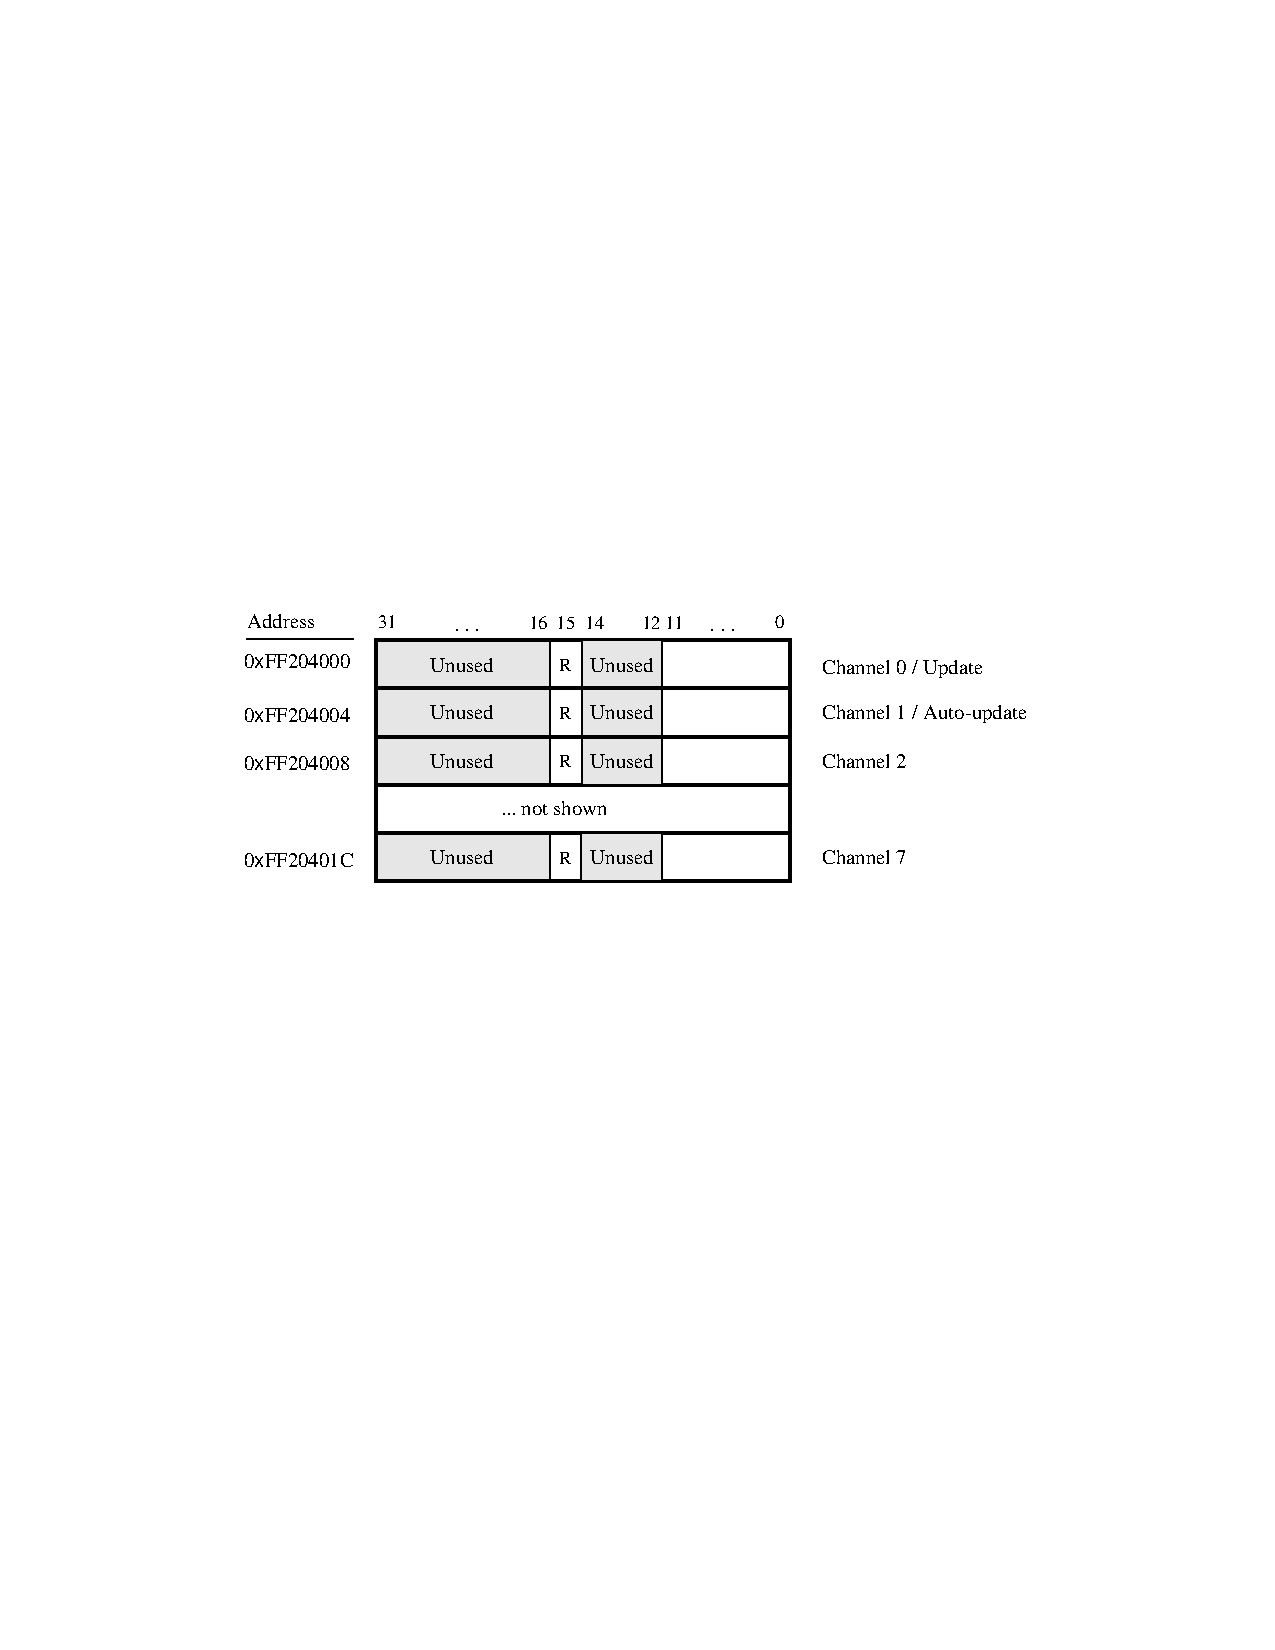
\includegraphics{figures/Media_FPGA_ADC.pdf}
   \end{center}
   \caption{ADC port registers.}
	\label{fig:ADC_port}
\end{figure}

\noindent
Figure~\ref{fig:ADC_conn} shows the connector on the DE1-SoC board that is used with the
ADC port. Analog signals in the range of 0 V to the $V_{CC5}$ power-supply voltage can be 
connected to the pins for channels 0 to 7. This connector is located on the left side of
the DE1-SoC board, near the power switch.

\begin{figure}[h!]
   \begin{center}
       \includegraphics{figures/fig_adc_conn.png}
   \end{center}
   \caption{ADC connector.}
	\label{fig:ADC_conn}
\end{figure}

\noindent
\section*{Part I}

\noindent
Write a C-language program to read the converted digital value on channel 0 of the ADC, and 
repeatedly print the value to the terminal. To verify that you are correctly reading the values,
try the following: 
\begin{itemize}
\item Use a wire to connect the {\it Ch}$_{0}$ pin to the \textit{Gnd} pin and see that the 
value read is equal, or very close, to zero.
\item Use the wire to connect {\it Ch}$_{0}$ to the power-supply value $V_{CC5}$ and verify that
the value read is equal, or very close, to 4095.
\item Note: to avoid possible damage to your board, be careful not to accidentally connect the
{\it Gnd} pin to the $V_{CC5}$ power pin.
\end{itemize}

\noindent
\section*{Part II}

\noindent
To test your oscilloscope, you will need to generate a signal to input into your oscilloscope. 
In this part, you will write a Linux* kernel module that will output a square wave onto a
parallel port. Your kernel module should create the waveform on pin $D_0$ of the parallel
port called JP1 in the DE1-SoC Computer. Connector JP1 is one of the large, 40-pin,
connectors on the board, and pin $D_0$ is at the top right corner of the connector.

~\\
\noindent
The frequency of the square wave generated by your kernel module should be configurable between
10 Hz to 160~Hz, in 10 Hz increments. The frequency is selected by the four leftmost switches on
the board, SW$_{9-6}$ (SW$_{3-0}$ for the DE10-Nano). An SW$_{9-6}$ value 
of \texttt{0000} would correspond to 10 Hz, \texttt{0001} to 20 Hz, and 
so on. To generate the square wave, your kernel module should use a {\it hardware timer}
to generate interrupts at regular intervals. You can use the interval timer implemented 
in the FPGA called {\it FPGA Timer0}. The register interface for this timer has the base 
address \texttt{0xFF202000}. As shown in Figure~\ref{fig:timer} this timer has six 16-bit 
registers. To use the timer you need to write a suitable value into the {\it Counter start value}
registers (there are two, one for the upper 16~bits, and one for the lower 16~bits of the 
32-bit counter value). To start the counter, you need to set the {\it START} bit in the 
{\it Control} register to~1. Once started the timer will count down to~0 from the initial 
value in the {\it Counter start value} register.  The counter will automatically reload this 
value and continue counting if the {\it CONT} bit in the {\it Control} register is~1. When the 
counter reaches~0, it will set the {\it TO} bit in the {\it Status} register to~1.
This bit can be cleared under program control by writing a~0 into it. If the 
{\it ITO} bit in the control register is set to~1, then the timer will generate an ARM* 
interrupt each time it sets the {\it TO} bit. The timer clock frequency is 100 MHz. 
The interrupt ID of the timer is 72. Follow the instructions in the tutorial {\it Using Linux 
on DE-Series Boards} to register this interrupt ID with the Linux kernel and ensure that it invokes 
your kernel module whenever the interrupt occurs.

\begin{figure}[htb]
	\begin{center}
	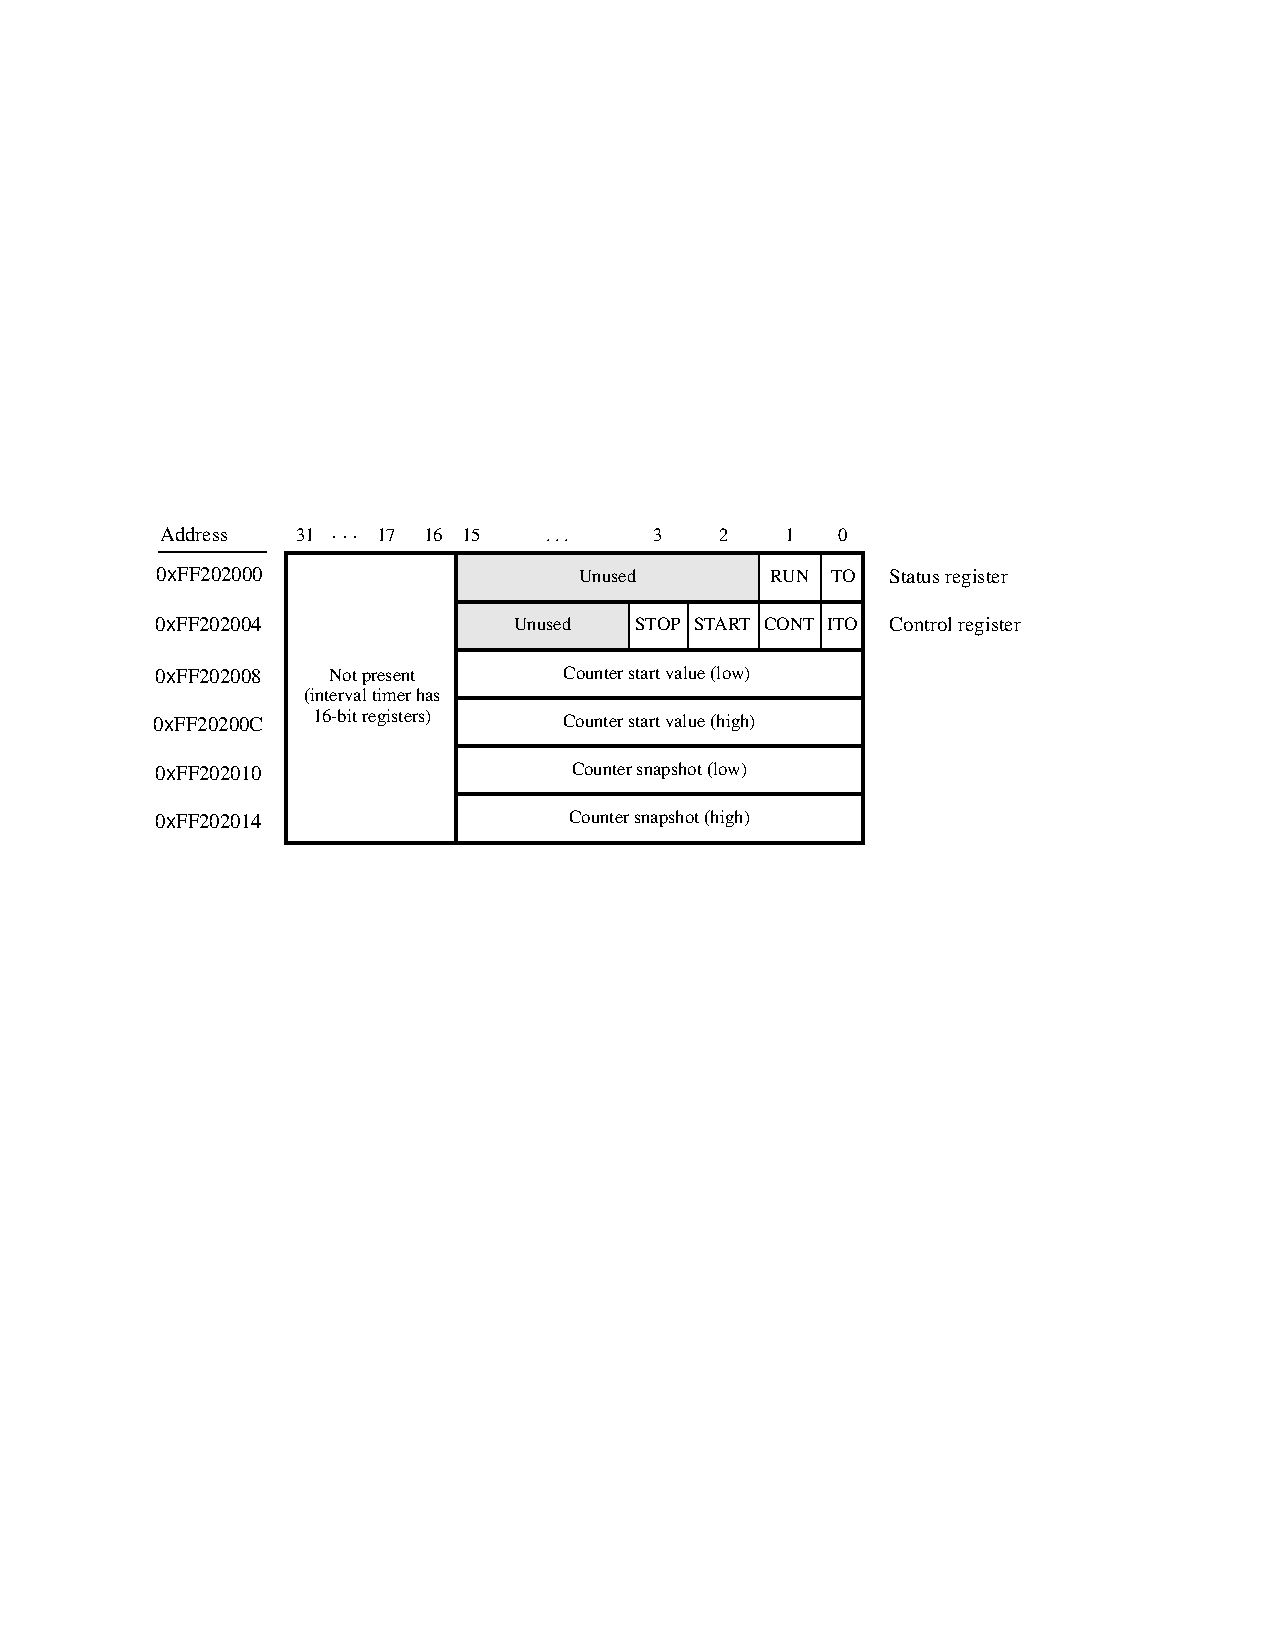
\includegraphics[scale=1]{figures/fig_interval_port.pdf}
	\end{center}
	\caption{The FPGA Timer0 register interface.}
\label{fig:timer}
\end{figure}

~\\
\noindent
The timer interval should equal half of the period of the square wave to be generated. 
Your interrupt handler should invert the value on pin $D_0$ of JP1
upon every interrupt, creating the desired square wave. Your interrupt handler 
should check to see if SW$_{9-6}$ have been altered, and adjust the square wave frequency as 
needed. An illustration of the programmer registers in a parallel port appears in
Figure~\ref{fig:parallel}.
It has a {\it data} register at an assigned {\it base} address. Each bit in this register could be
either an input or output, depending on the contents of the {\it direction} register. Setting
a bit in the direction register to 1 makes the corresponding data bit an output, while 0
makes it an input. The
{\it interruptmask} and {\it edgecapture} registers shown in the figure allow the port to
generate ARM processor interrupts. For this exercise, you need to use only the data and
direction registers. The base address of port JP1 is \texttt{0xFF200060}. Connector JP1 
(and JP2) is a 40-pin connector located on the right-hand side of the DE1-SoC board. As
mentioned before pin $D_0$ is at the top right corner of the connector.

~\\
\noindent
Perform the following:

\begin{enumerate}
\item Create a file called {\it signal\_generator.c} and write your kernel module in this file.

\item Your kernel module should show the values of the SW switches on the red lights LEDR. 
Also, it should show the value of the waveform frequency, which is a number between \red{10}
and \red{160}, on the seven-segment displays HEX3-HEX0 (if available on your board). 
Figures~\ref{fig:SW}-\ref{fig:HEX}
show the programming registers in the switch, light, and seven-segment display ports.

\item Create a Makefile, compile your kernel module, and insert it into the kernel. 
\end{enumerate}

\begin{figure}[htb]
	\begin{center}
	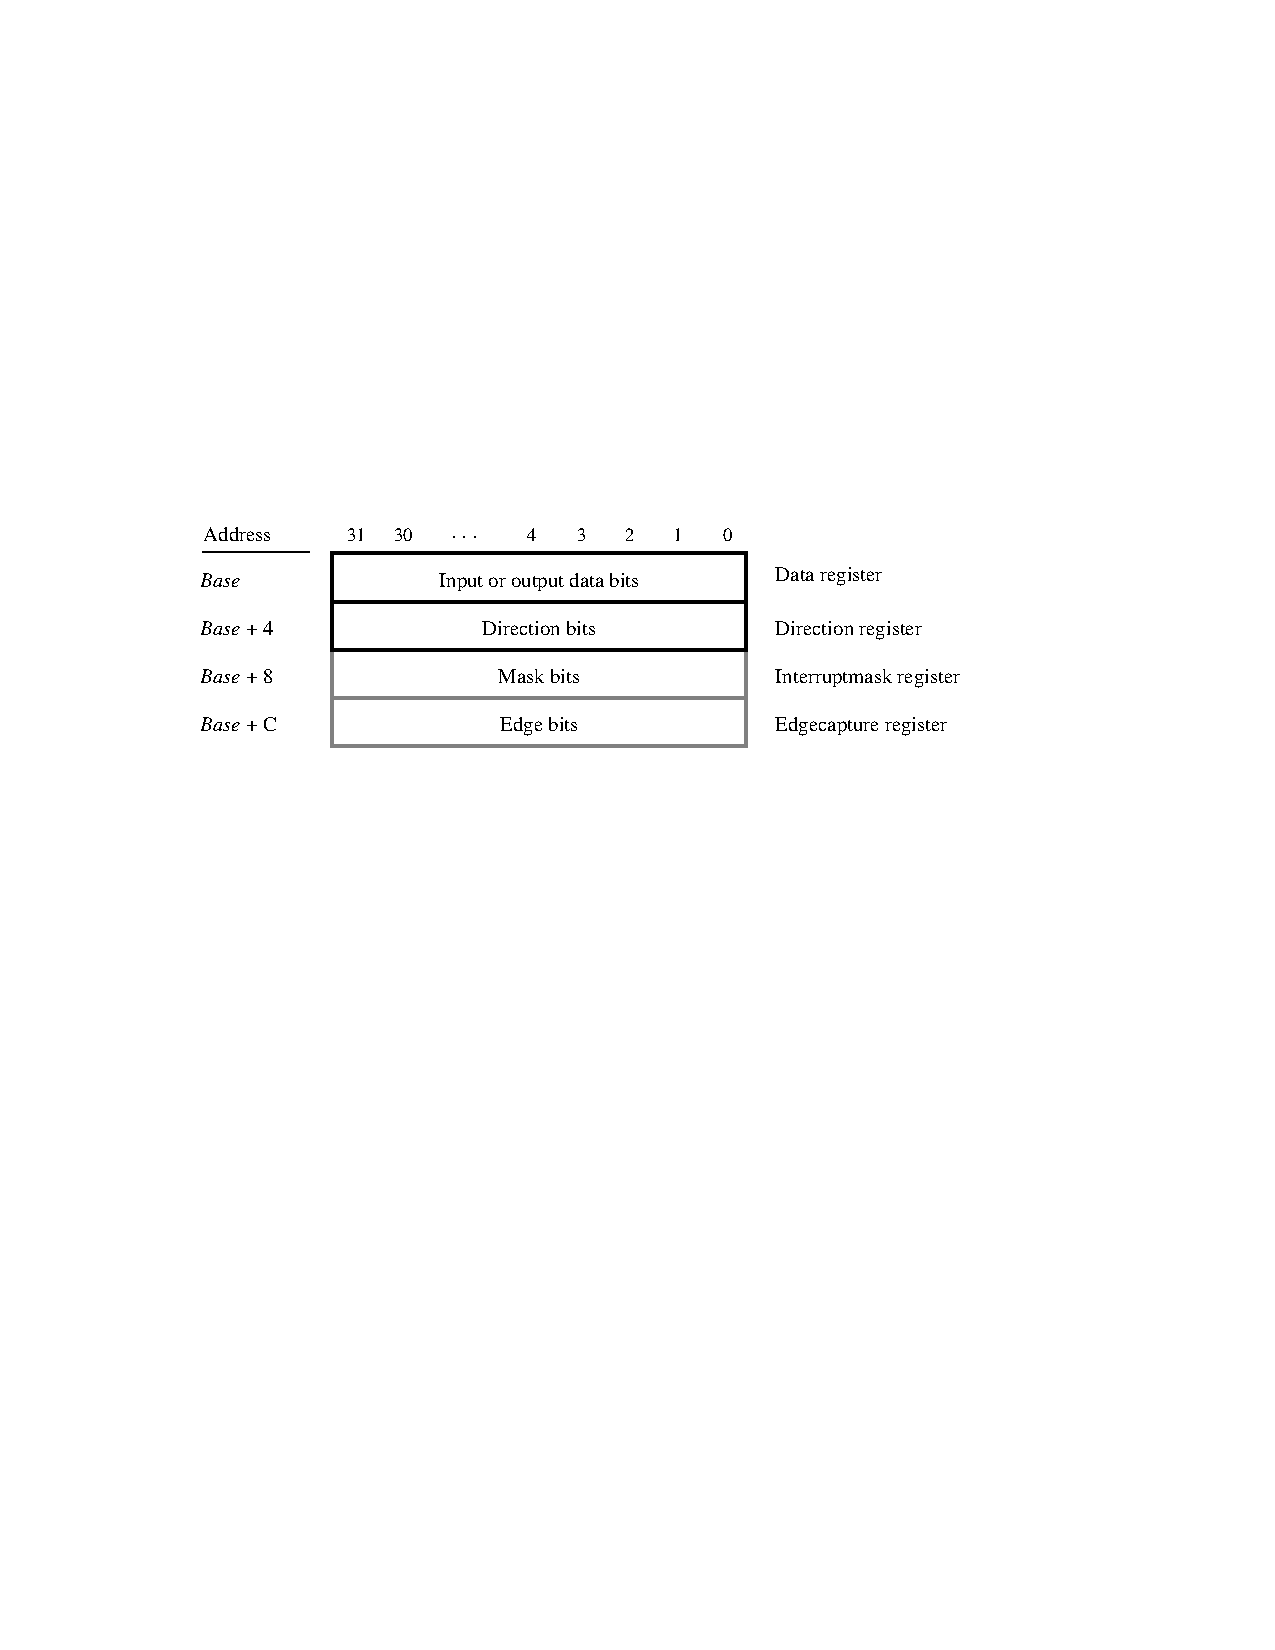
\includegraphics[scale=1]{figures/figureparallel.pdf}
	\end{center}
	\caption{The programming registers in a parallel port.}
\label{fig:parallel}
\end{figure}

\begin{figure}[htb]
	\begin{center}
	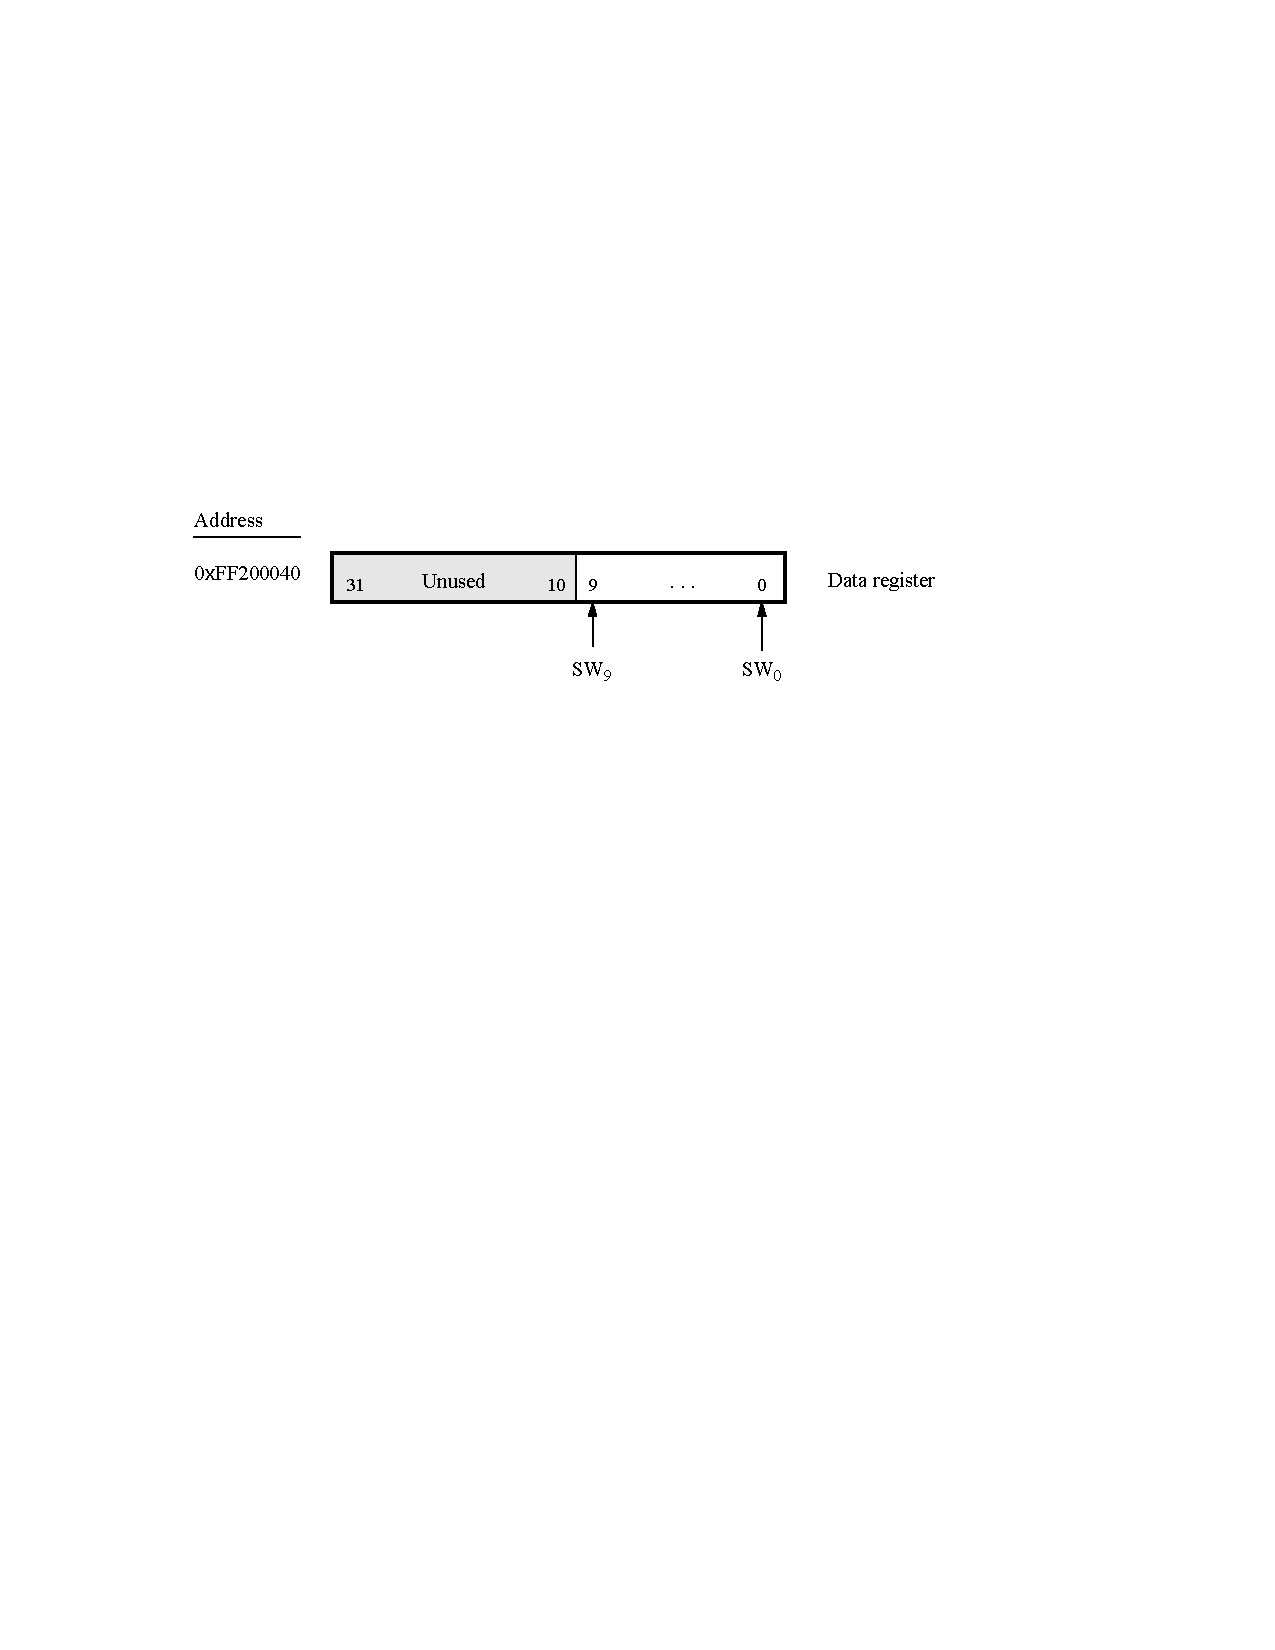
\includegraphics[scale=1]{figures/fig_slider_port.pdf}
	\end{center}
	\caption{The SW switch port.}
\label{fig:SW}
\end{figure}
\begin{figure}[htb]
	\begin{center}
	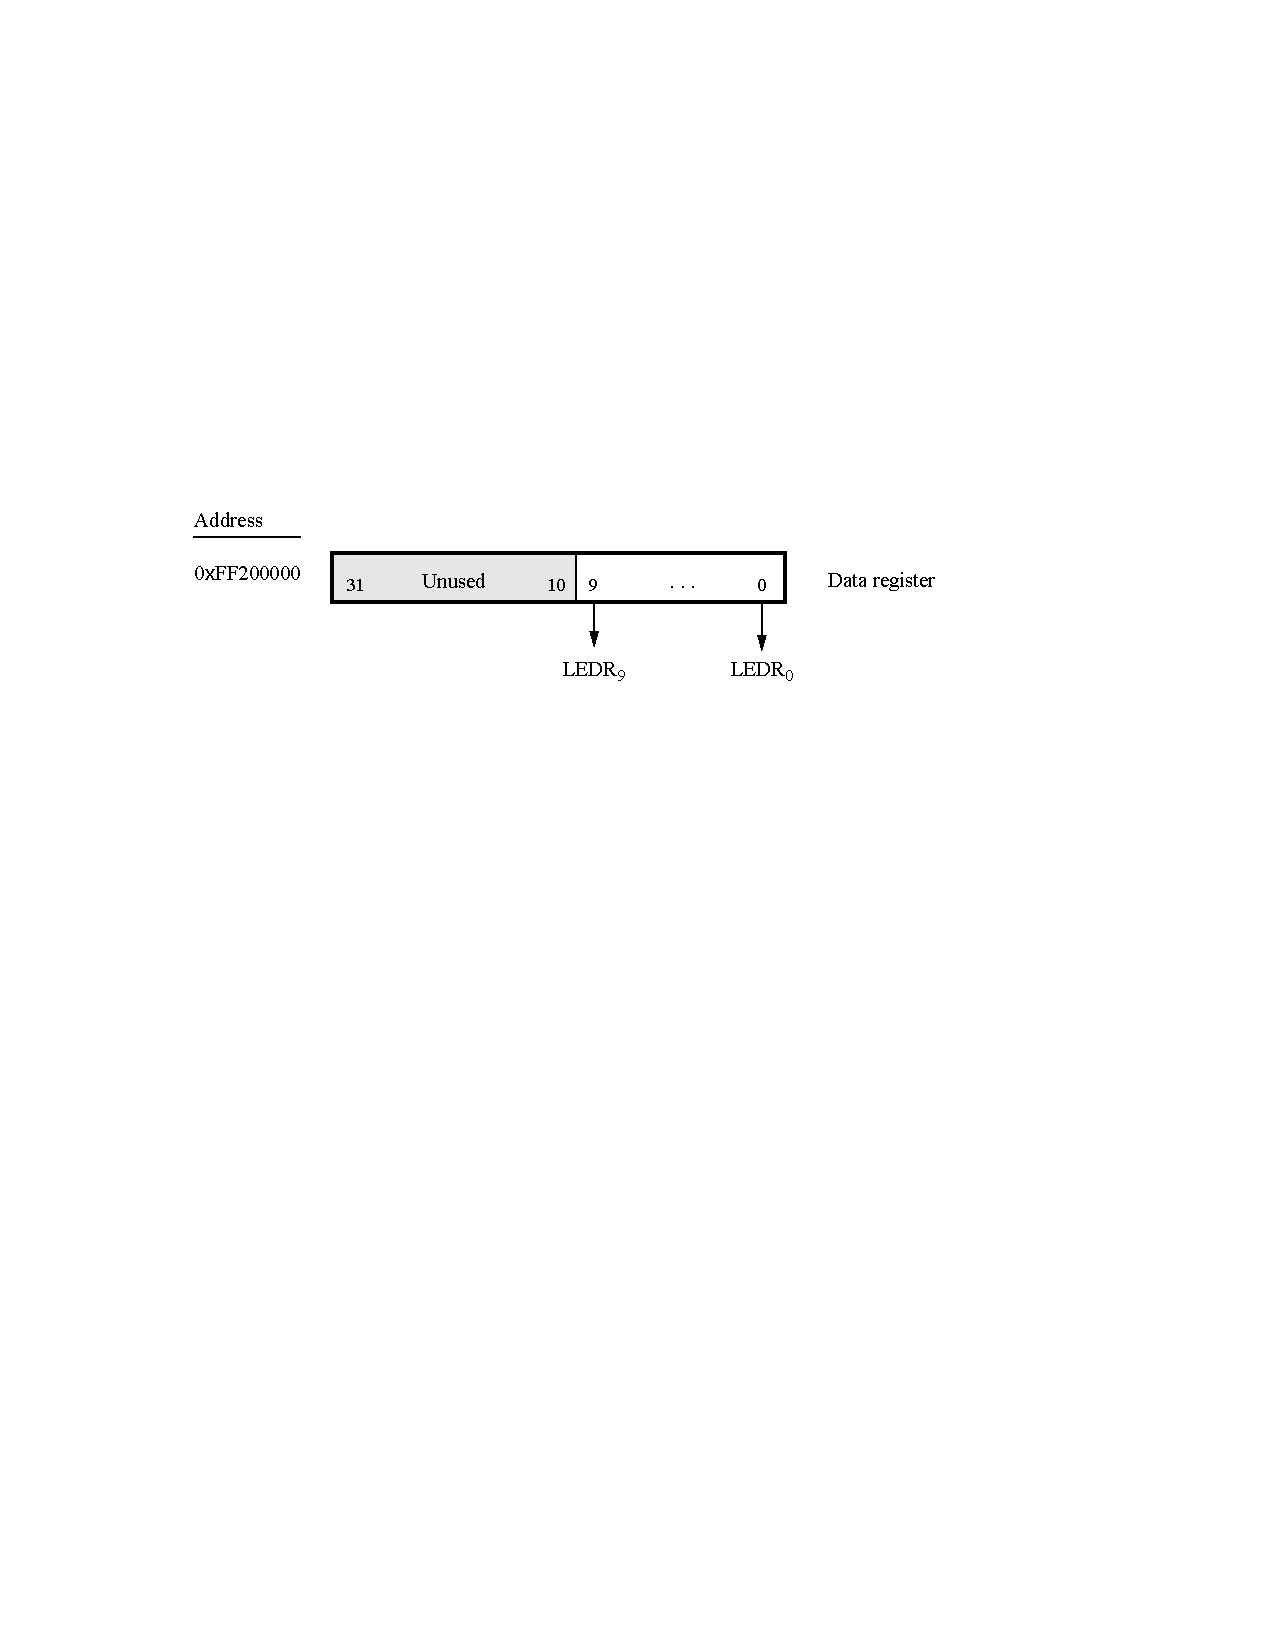
\includegraphics[scale=1]{figures/fig_LED_port.pdf}
	\end{center}
	\caption{The LEDR light port.}
\label{fig:LEDR}
\end{figure}

\begin{figure}[htb]
	\begin{center}
	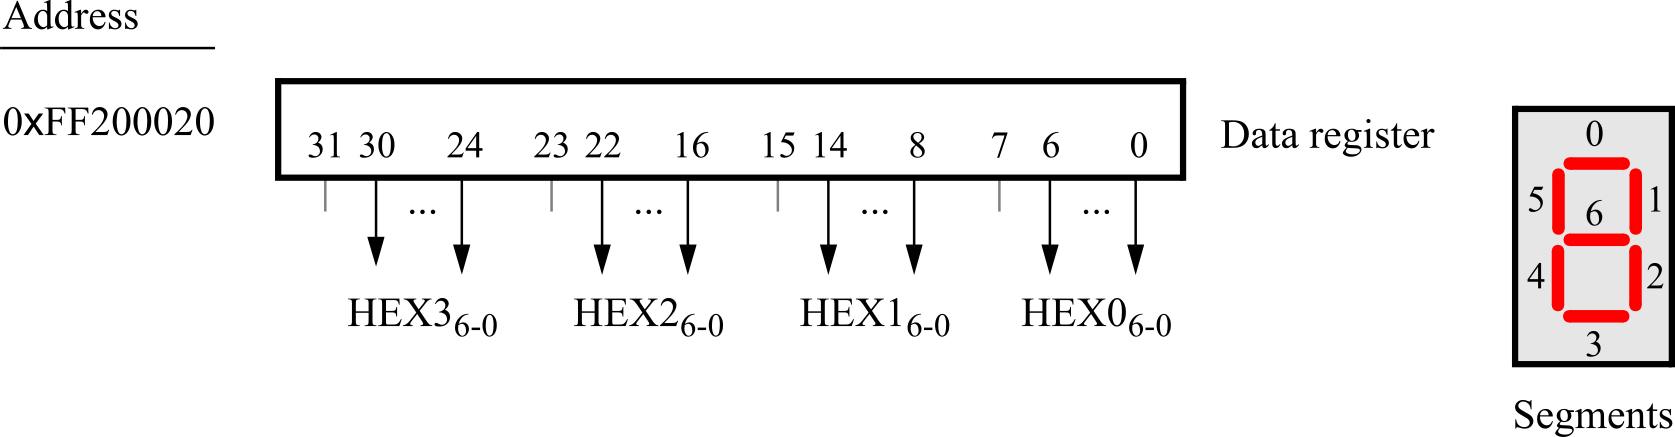
\includegraphics[scale=1]{figures/figureHEX.png}
	\end{center}
	\caption{The HEX seven-segment display ports.}
\label{fig:HEX}
\end{figure}

\noindent
\section*{Part III}

In this part you will write a C-language program to implement your oscilloscope.
Your program will sample the input waveform on channel 0 of the ADC, 
and display the signal graphically on the VGA output. The x-axis on the display will represent 
a timespan of 100 ms, and the y-axis will represent a voltage range of 0~V to 5~V. 

~\\
\noindent
An oscilloscope samples the input signal for some defined period of time, then displays that
stretch of recorded data on the screen. This stretch of data capture is referred to as the
{\it sweep}. Your oscilloscope will have a sweep of 100 ms. A sweep should start when
the oscilloscope detects one of two triggers: a rising edge of the square wave, or a falling edge 
of the square wave. Switch SW$_0$ should control which of the two triggers is to be detected, 
with position 1 selecting the rising edge, and 0 the falling edge. Upon completing each sweep, 
your oscilloscope will draw the newly captured waveform on the display, then re-arm the trigger
to start another sweep as soon as the next trigger is detected.

~\\
\noindent
During a sweep your oscilloscope should capture one sample for each $x$ coordinate of the 
VGA display. The samples should be captured in regular intervals. For example, if
$x=320$, then a sample should be captured every 100 ms / 320 = 0.3125~ms. To capture data 
at regular intervals, you will need to use an interval timer like you did in Part II. However,
instead of directly controlling a hardware timer using its register interface, you will use 
a Linux application programmer interface (API) for creating and using timers. This API allows 
you to create and set an interval timer which will send a {\it signal} to your program upon 
each timeout. As part of your program, you can implement a {\it handler} function for the signal to 
capture a sample on each timeout. The timer API is provided by the library \texttt{<time.h>}, 
and its use is illustrated in Figure~\ref{fig:timer_code}. When compiling, you must add the 
flag "-lrt" to the end of your \texttt{gcc} command to link in the \textit{Realtime} library 
which includes \texttt{<time.h>}. 

\newpage
Key lines of code are described below:

\begin{itemize}
\item Lines~\ref{line:inc1}-\ref{line:inc2}: The header files that provide the timer 
functions.
\item Lines~\ref{line:t1}-\ref{line:t2}: The timer specification structure which is used to set the timer to count 0.3125 ms intervals. The \texttt{it\_interval} variable specifies when the initial timeout occurs after setting the timer (set to 312500 ns, which equals 0.3125 ms). The \texttt{it\_value} variable specifies the repeating timeout interval after the initial timeout.
\item Lines~\ref{line:ts1}-\ref{line:ts2}: The timer specification structure for stopping a timer. Notice that the variables are set to 0, which turns off the timer.
\item Lines~\ref{line:f1}-\ref{line:f2}: The function that handles a timer timeout. This function is called every 0.3125 ms. 
\item Line~\ref{line:sig2}: Registering the function \texttt{timeout\_handler($\ldots$)} as 
the handler for the \texttt{SIGALRM} signal. Our timer generates the 
\texttt{SIGALRM} signal upon each timeout, thus invoking the
\texttt{timeout\_handler($\ldots$)} function at the desired frequency.
\item Line~\ref{line:mono}: Creates a monotonically increasing timer. At this point, the timer is inactive.
\item Line~\ref{line:timer}: Arms the timer, making it timeout every 0.3125 ms. Upon each 
timeout, the timer will send the \texttt{SIGALRM} signal to this program, which will invoke 
the \texttt{timeout\_handler($\ldots$)} function.
\item Line~\ref{line:stop}: Stops the timer by configuring it with a zero for both 
\texttt{it\_interval} and \texttt{it\_value}.
\end{itemize}

\noindent
In your oscilloscope program, whenever a trigger condition is satisfied you should call the 
function \texttt{timer\_settime} as shown in line~\ref{line:timer} to start a sweep. After the
samples for the sweep have been collected by your timeout handler, you should 
call \texttt{timer\_settime} again, as illustrated in line~\ref{line:stop}, to stop the timer.

~\\
\noindent
Perform the following:

\begin{enumerate}
\item Create a C program that implements your oscilloscope.

\item Compile your program, appending the required flag "-lrt" to your \texttt{gcc} command 
so that it links in the \textit{Realtime} library. For instance, if your source-code is
stored in a file {\it part3.c}, then an appropriate command would be 
\texttt{gcc -o part3 part3.c -lrt}.

\item Ensure that pin $D_0$ of connector JP1 is connected to {\it Ch}$_0$ of the ADC, and that
your kernel module from Part II is inserted into the Linux kernel. Run your oscilloscope
program and observe the VGA display. Try toggling SW$_{9-6}$ and observe the change in the 
displayed waveform. The oscilloscope's display should look similar to 
Figure~\ref{fig:part2_screenshot}. In this figure, the waveform has a frequency of 100 Hz, 
as 10 periods of the signal are visible within the 100 ms span. Since the JP1 pins operate 
at 3.3 V, the waveform spans roughly $2 \over 3$ of the 5~V vertical range.
\end{enumerate}

\lstset{language=C,numbers=left,escapechar=|}
\begin{figure}[H]
\begin{center}
\begin{minipage}[t]{16 cm}
\begin{lstlisting}
|\label{line:inc1}|#include <signal.h>
|\label{line:inc2}|#include <time.h>
|$\ldots$|
|\label{line:t1}|struct itimerspec interval_timer_start = {
	.it_interval = {.tv_sec=0,.tv_nsec=312500},
|\label{line:t2}|	.it_value    = {.tv_sec=0,.tv_nsec=312500}};
|\label{line:ts1}|struct itimerspec interval_timer_stop  = {
 	.it_interval = {.tv_sec=0,.tv_nsec=0},
	|\label{line:ts2}|.it_value    = {.tv_sec=0,.tv_nsec=0}};
timer_t interval_timer_id;

|\label{line:f1}|// Handler function that is called when a timeout occurs
void timeout_handler(int signo) {
	|$\ldots$| code not shown 
|\label{line:f2}|}
int main(void)
{
	|$\ldots$| 
	|\label{line:sig1}|// catch SIGALRM and call the handler
	|\label{line:sig2}|signal(SIGALRM, timeout_handler);

	// Create a monotonically increasing timer
	|\label{line:mono}|timer_create (CLOCK_MONOTONIC, NULL, &interval_timer_id);
	|$\ldots$|
	// Starting the timer
	|\label{line:timer}|timer_settime (interval_timer_id, 0, &interval_timer_start, NULL);
	|$\ldots$|
	// Stopping the timer
	|\label{line:stop}|timer_settime (interval_timer_id, 0, &interval_timer_stop, NULL);
}
\end{lstlisting}
\end{minipage}
\end{center}
\vspace{-0.25in}\caption{Using the timer functions.}
\label{fig:timer_code}
\end{figure}

\begin{figure}[H]
   \begin{center}
			  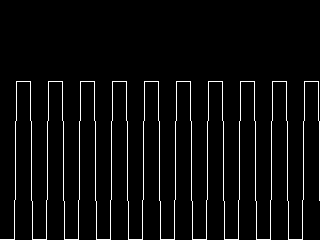
\includegraphics[scale=0.8]{figures/part2_screenshot.png}
   \end{center}
   \caption{Screenshot of the oscilloscope program's video output.}
	\label{fig:part2_screenshot}
\end{figure}

\noindent
\section*{Part IV}

Oscilloscopes usually have a sweep control function that allows a user to control the
sweep duration. Add such a function to your oscilloscope, by using the KEY inputs of the
DE1-SoC Computer. Pressing KEY$_0$ should cause the sweep time to increase by 100 ms, and
pressing KEY$_1$ should decrease the sweep time. Figure~\ref{fig:KEY} shows the
programming registers in the KEY port. When a KEY is pressed, the corresponding 
bit-position in both the {\it Data} and {\it Edgecapture} registers is set to 1. The {\it Data}
register bit is cleared as soon as the KEY is released, while the {\it Edgecapture} 
register bit remains set until manually cleared under program control. An {\it Edgecapture}
register bit can be cleared by writing a 1 into it.

\begin{figure}[htb]
	\begin{center}
	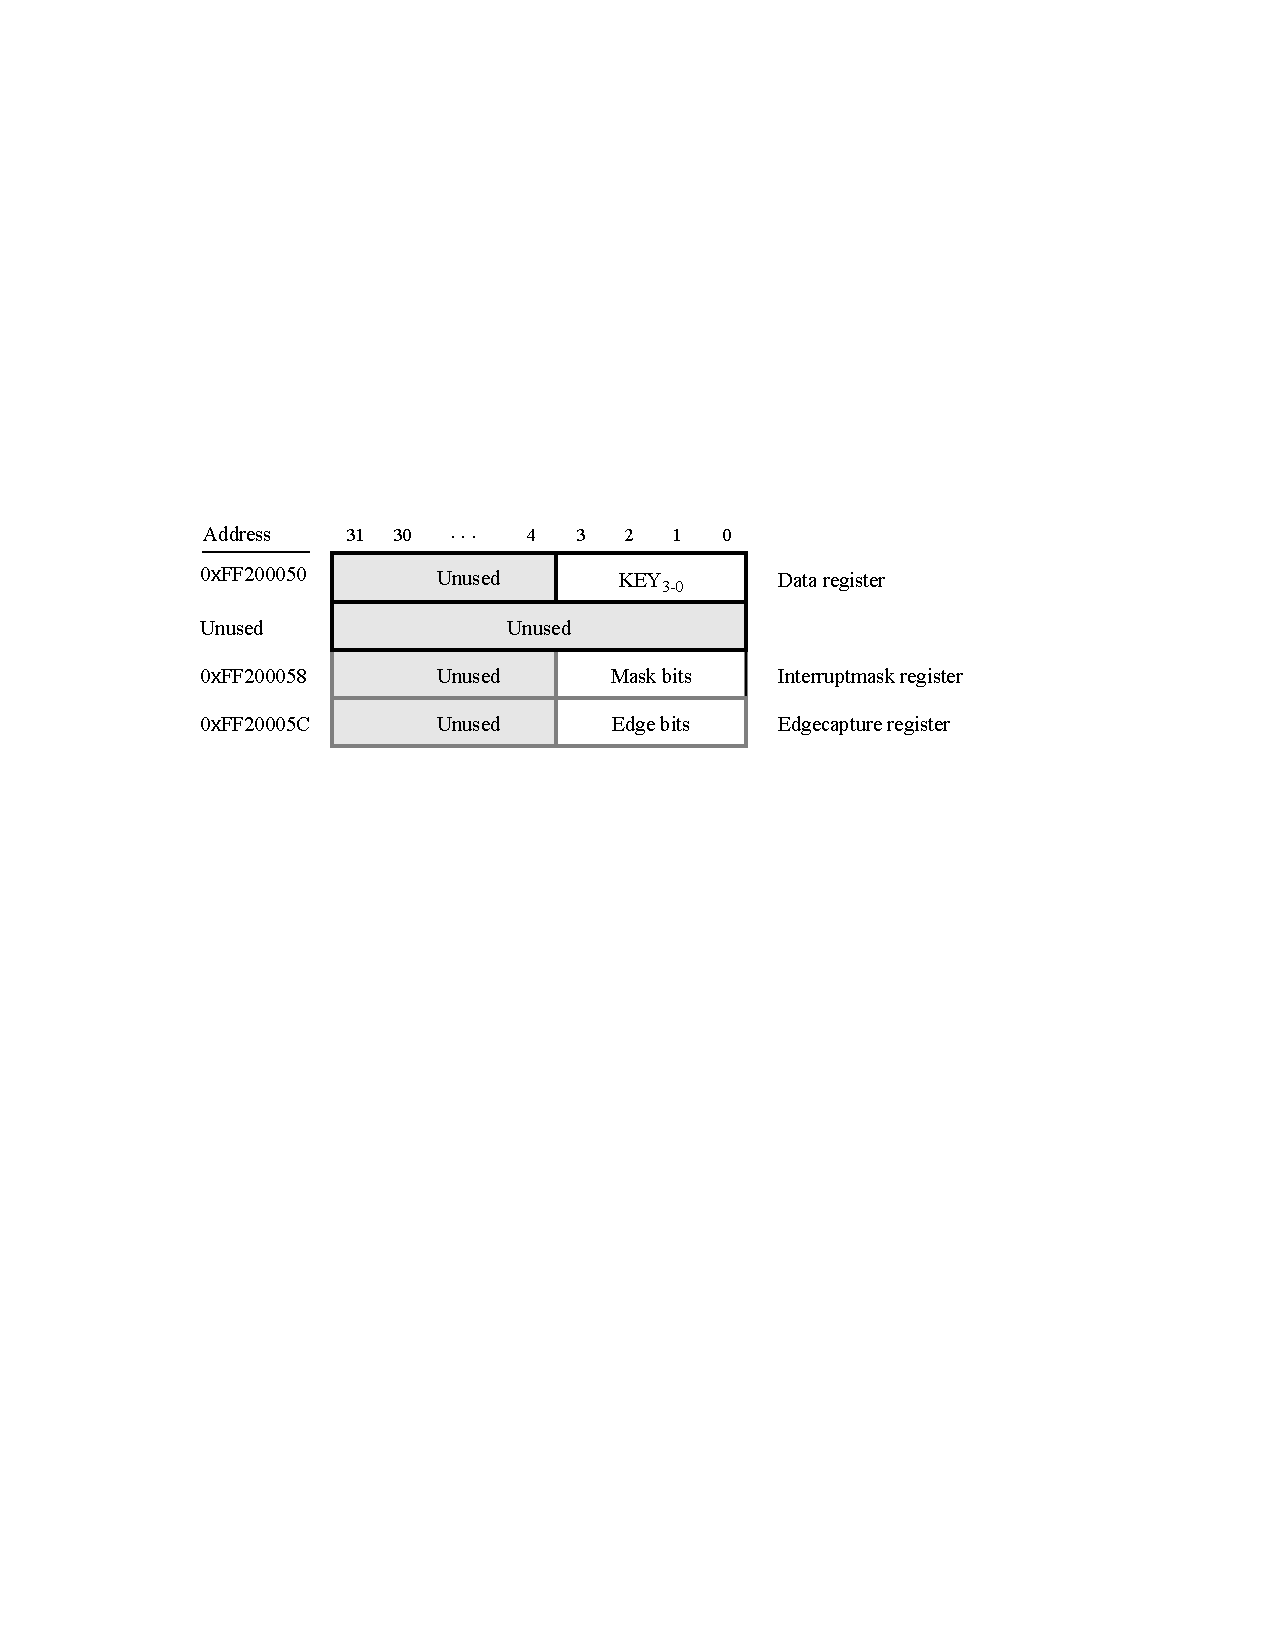
\includegraphics[scale=1]{figures/figureKEY.pdf}
	\end{center}
	\caption{The KEY port.}
\label{fig:KEY}
\end{figure}

\vskip 0.8in
\noindent
\newpage
%%%%%%%%%%%%%%%%%%%%%%%%%%%%%%%%%%%%%%%%
%%% FPGAcademy Copyright Information %%%
%%%%%%%%%%%%%%%%%%%%%%%%%%%%%%%%%%%%%%%%

%Always put the copyright on a new page (clear page), with some vertical space from top
\clearpage
\vspace{1in}

\noindent

Copyright {\copyright} FPGAcademy.org. All rights reserved. FPGAcademy and the 
FPGAcademy logo are trademarks of FPGAcademy.org.  This document is provided 
"as is", without warranty of any kind, express or implied, including but not 
limited to the warranties of merchantability, fitness for a particular purpose 
and noninfringement. In no event shall the authors or copyright holders be 
liable for any claim, damages or other liability, whether in an action of 
contract, tort or otherwise, arising from, out of or in connection with the 
document or the use or other dealings in the document.
~\\
~\\
**Other names and brands may be claimed as the property of others.


\end{document}
